\chapter{Introdução}

Em outubro de 2023, Manaus liderou a lista das cidades com a pior qualidade do ar no mundo, apresentando nuvens de fumaça em alguns dias do mês. Segundo a prefeitura da capital amazonense, essa situação foi resultado da intensa onda de queimadas na região \cite{G1-ar-manaus}. Diante do cenário descrito, uma preocupação relevante é a intoxicação por inalação de gases asfixiantes, como o monóxido de carbono (CO). O gás, presente no ar devido à combustão incompleta de materiais ricos em carbono, é uma substância tóxica, incolor e inodora, que atua no organismo da seguinte forma: ao se ligar quimicamente à hemoglobina, proteína no sangue responsável pelo transporte de oxigênio, com uma afinidade 200 a 300 vezes maior que a ligação do oxigênio ($O_{2}$), o monóxido de carbono reduz a eficiência do transporte de oxigênio no organismo e pode levar a óbito caso haja exposição prolongada e altas quantidades \cite{carbon-monoxide-poisoning-varon}.

No ambiente doméstico, as fontes mais comuns do gás CO são: aquecedores, fogões, automóveis em garagens pouco ventiladas, entre outros. Outro fator de risco é o vazamento devido ao mau uso e/ou à falta de manutenção dos equipamentos, pois a detecção do gás antes do início dos sintomas é dificultada sem equipamentos de medição adequados \cite{bio-sufocantes-hernandez2022}. Portanto, decidiu-se abordar a problemática por meio de um sistema Android embarcado, com foco na emissão de alertas de risco aos ocupantes. O projeto de trabalho de conclusão de curso consiste na elaboração e desenvolvimento de um protótipo de \textit{hardware}, em conjunto com o \textit{software} necessário na interação do usuário com os outros módulos do sistema. 

\section{Objetivos}

O objetivo geral do trabalho é oferecer uma solução embarcada para o monitoramento da qualidade do ar em ambiente residencial, com ênfase na coleta de dados e identificação de condições de risco, pois proporcionar aos ocupantes do imóvel informações cruciais sobre a qualidade do ar interno contribui na adoção de medidas preventivas.

Portanto, para alcançar o objetivo geral, é necessário cumprir os seguintes objetivos específicos:
\begin{itemize}
    \item Elaborar pesquisa com usuários e avaliação do sistema;
    \item Coletar, compreender e tratar as informações dos sensores de: monóxido de carbono, temperatura e umidade do ar;
    \item Construir o protótipo do dispositivo embarcado;
    \item Realizar a comunicação entre o dispositivo e os demais módulos da aplicação;
    \item Desenvolver a API de dados e eventos, assim como a interface do sistema com o usuário;
\end{itemize}

\section{Justificativa}

O projeto visa contribuir para o monitoramento e detecção de riscos de intoxicação de gás em residências, cujo impacto se manifesta na prevenção de acidentes, tomada de decisão com apoio de dados e também na automatização de sinais de alerta. Outro ponto de destaque da importância desse trabalho diz respeito ao risco de morte por asfixia que a substância monóxido de carbono possui, pois sua presença não é detectada pelo olfato humano e o tempo de exposição é um fator determinante para os efeitos na saúde. 

A diminuição no fornecimento de oxigênio causa consequências graves ao organismo, indo desde sintomas brandos como náusea e dores de cabeça até casos mais sérios como, por exemplo, lesão neurológica e disritmia cardíaca \cite{carbon-monoxide-poisoning-varon}. Esta perspectiva enriquece a contribuição do trabalho no campo de IoT e ressalta a importância do uso de sistemas inteligentes para o monitoramento ambiental. A implementação de sensores capazes de detectar níveis perigosos de gases tóxicos como o monóxido de carbono pode prevenir acidentes graves e salvar vidas, pois proporciona ao usuário o conhecimento de situações potencialmente fatais. 

\section{Metodologia}

A metologia de trabalho baseia-se no fluxo de atividades \textit{embedded design life cycle diagram} \cite{system-design-IOT}. O diagrama possui vantagem no particionamento de atividades em \textit{hardware} (HW) e \textit{software} (SW), pois favorece a execução de tarefas paralelas dentro do mesmo escopo, sendo positivo para sistemas embarcados e suas restrições intrínsecas, como alto acoplamento e dependência entre componentes. A execução simultânea de atividades em duas áreas permite a validação de funcionalidades do sistema nas entregas incrementais e otimização do processo de desenvolvimento. O método original possui 7 fases principais:  

\begin{enumerate}
    \item Especificação do produto;
    \item Particionamento em componentes de hardware e software;
    \item Iteração e refinamento das funcionalidades;
    \item Atividades de hardware e software;
    \item Integração de componentes;
    \item Testes de aceitação e lançamento do produto;
    \item Manutenção e atualização do produto final;
\end{enumerate}

Contudo, o método trata do desenvolvimento de produto (e não de uma pesquisa acadêmica). Dito isso, o processo sofreu as seguintes alterações para adaptação ao contexto da universidade: a primeira fase deverá conter a pesquisa de trabalhos relacionados e domínio do problema, enquanto sua última etapa trata de documentação e escrita da monografia, como resultado do trabalho de conclusão de curso. Portanto, a seguinte figura demonstra a metodologia utilizada na execução do projeto: 

\begin{figure}[ht]
\centering
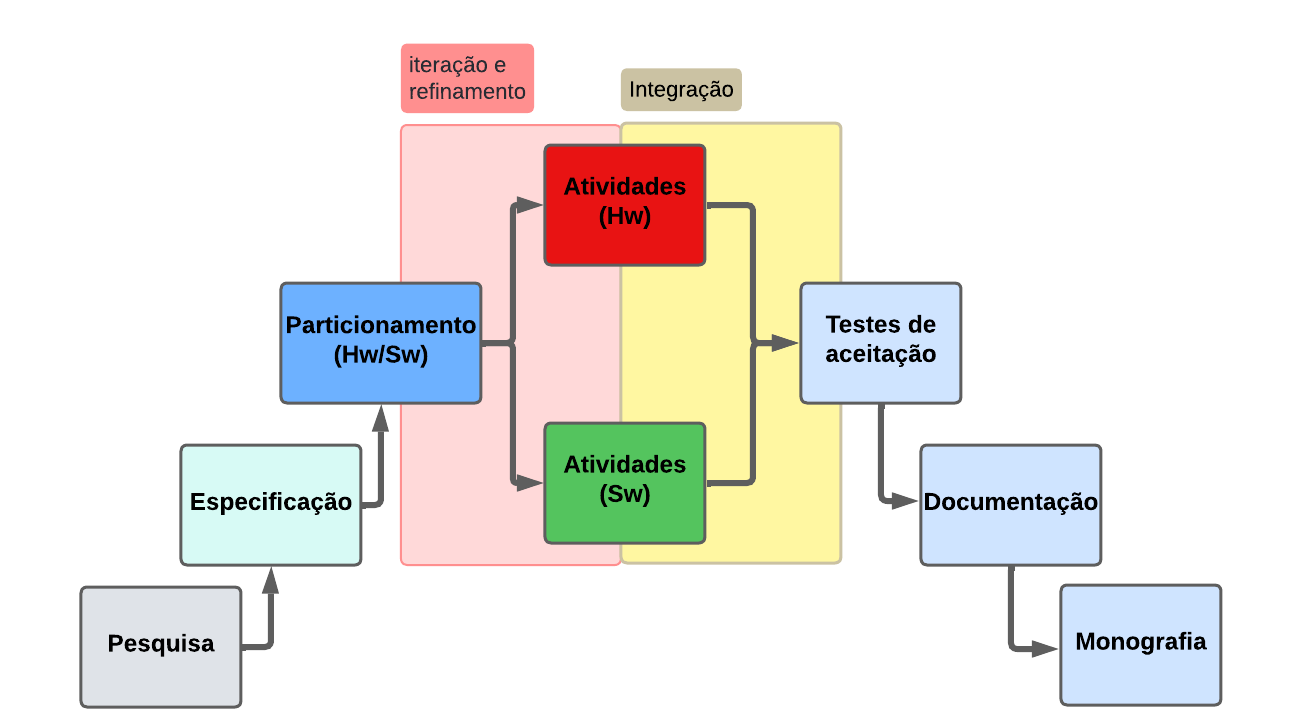
\includegraphics[width=.75\textwidth]{img/diagrama-metodologia.png}
\caption{Fluxo de atividades. Fonte: Elaboração própria com base  em\cite{system-design-IOT}}\label{figMetodologia}
\end{figure}

A fase de pesquisa consiste na busca de trabalhos relacionados sobre o tema de interesse, onde ocorre a avaliação crítica de cada projeto e seus pontos de melhoria, assim como um estudo detalhado do gás monóxido de carbono. Em seguida, o estudo da medição de concentração do gás e levantamento dos componentes eletrônicos para a montagem do protótipo físico. Ao final, o domínio do problema será abordado na pesquisa por entrevistados e suas especificidades no ambiente residencial. 

Em segundo, existe a fase de especificação. Ocorre o levantamento de funcionalidades do sistema, com aplicação de questionário e entrevistas para a compreensão do fenômeno observado. Por outro lado, é realizada também a modelagem do circuito eletrônico, arquitetura do \textit{software} de dados/alertas, fluxo de navegação do aplicativo móvel e, por fim, o planejamento da comunicação entre o aplicativo e a biblioteca customizada no \textit{AOSP}. 

O particionamento em componentes de \textit{hardware} e \textit{software} (Hw/Sw) marca o início do processo iterativo. O terceiro processo identifica as funcionalidades do escopo e leva em consideração a dependência entre os serviços que as diferentes camadas do sistema provêm.

O quarto item do fluxo define as atividades necessárias para a entrega da funcionalidade descrita em fases anteriores. Além da definição, a lista de atividades passa por um refinamento para eliminar ambiguidade e inconsistência. Em atividades de \textit{software} e \textit{hardware} ocorre a simples execução das tarefas. Na sexta etapa, haverá a integração entre os componentes gerados na execução de atividades, verificando casos de teste para verificar o comportamento adequado da entrega parcial, caso contrário os artefatos deverão ser revistos para identificar a causa do problema. O ciclo funciona até finalizar todas as entregas parciais do produto.

Os testes de aceitação e lançamento do protótipo serão realizados com os usuários finais do sistema. A fase consiste em identificar dificuldades em configurar o aparelho, uso de aplicativo, notificações e disparo de alertas para, ao final, identificar fatores na interação com o sistema que representam certa dificuldade. Em penúltimo, a manutenção do sistema e atualização do protótipo é o momento em que todo o projeto será estruturado para o uso do público geral, assim como a confecção do guia de instalação. Por fim, a última etapa consiste na escrita da monografia e consolidação dos resultados obtidos.